\chapter{Soporte de TurtleBot2 en ROS Foxy}
\label{cap:capitulo4}

% -- INTRODUCCION
% -----------------
En este capítulo se presenta el proceso de migración del robot TurtleBot2 de ROS Noetic a ROS2 Foxy. Se describirán todos los cambios relevantes realizados como puede ser la modificación de sus ficheros URDF/Xacro, su lanzamiento en Gazebo a través de los \textit{launchers} de ROS2 o incluso su integración sobre una imagen Docker.\\

El soporte del robot en ROS2 Foxy supuso el primer paso del proyecto para desarrollar los nuevos ejercicios de Robotics Academy con este robot\\




% -- SECCION ROBOT SIMULADO
\section{Robot TurtleBot2 simulado en Gazebo}
\label{sec:robot_simulado_gazebo}
El soporte más estable del TurtleBot2 se encuentra en la rama de ROS Melodic (tanto real como simulado) aunque también funciona en ROS Noetic \footnote{\textbf{TurtleBot 2 (Noetic)}: \url{https://bitbucket.org/theconstructcore/turtlebot/src/noetic/}}. Sin embargo, para ROS2 Foxy solamente hay un repositorio \footnote{\textbf{Base Kobuki (foxy)}: \url{https://github.com/kobuki-base/kobuki_ros}} que actúa de \textit{wrapper} con el driver del robot real (veremos más en la sección \ref{sec:robot_real_ros_foxy}). De modo que en esta sección abarcaremos el proceso de modelado del cuerpo del robot y la creación de los ficheros de lanzamiento para Gazebo.\\


\subsection{Base Kobuki}
\label{subsec:kobuki_base_simulado}

El repositorio oficial de la base Kobuki contiene un paquete denominado \textit{kobuki\_description}, que contiene los ficheros de descripción Xacro (Sección \ref{subsec:xacro}) y URDF (Sección \ref{subsec:urdf}) de la base. En estos ficheros se describe el árbol de tranformadas que existen entre todos los \textit{links} (tramos, partes) del robot, y de esta manera conocer la localización de todos los marcos de coordenadas. También se añaden \textit{plugins} para facilitar el control de movimiento del robot (controladores de velocidad, odometría ...). Sin embargo, este paquete carece de ficheros de lanzamiento para el simulador, de modo que tuvimos que diseñar nuestros propios \textit{launchers}.\\

Para conseguir la representación de la base Kobuki en Gazebo hicimos un copia\footnote{\textbf{Kobuki ROS (fork)}: \url{https://github.com/Carlosalpha1/kobuki_ros}} del repositorio oficial e implementamos un nuevo paquete llamado \textit{kobuki\_gazebo}. Dentro se incluyeron ficheros \texttt{launch.py} para lanzar tanto el simulador como la base kobuki simulada. A continuación describiremos los ficheros más importantes del nuevo paquete implementado:

\begin{itemize}
	\item \textbf{empty\_world.launch.py}: Un punto de partida en muchas ocasiones cuando creamos un robot simulado es diseñar un fichero de lanzamiento que únicamente lance un mundo vacío en Gazebo. De esta manera, puedes incluir ese fichero en otros ficheros de lanzamiento y dividimos un problema complejo en varios subproblemas. Para lanzar Gazebo en ROS2 ejecutamos dos ficheros de lanzamientos en este orden:
	\begin{enumerate}
		\item gazebo\_ros - \texttt{gzserver.launch.py}: Lanza un servidor de Gazebo sin ventana gráfica, permitiendo ejecutar programas sin necesidad de visualizar el resultado en el simulador.
		\item gazebo\_ros - \texttt{gzclient.launch.py}: Lanza un cliente de Gazebo que activa una ventana gráfica donde podemos ver el mundo solicitado.
	\end{enumerate}

\begin{code}[H]
\begin{lstlisting}[frame=single]
def generate_launch_description():

	ld = LaunchDescription()

	pkg_gazebo_ros = get_package_share_directory('gazebo_ros')
		
	gazebo_server = IncludeLaunchDescription(
		PythonLaunchDescriptionSource(os.path.join(pkg_gazebo_ros, 'launch', 'gzserver.launch.py'))
	)
		
	gazebo_client = IncludeLaunchDescription(
		PythonLaunchDescriptionSource(os.path.join(pkg_gazebo_ros, 'launch', 'gzclient.launch.py'))
	)
	
	ld.add_action(gazebo_server)
	ld.add_action(gazebo_client)
	
	return ld
\end{lstlisting}
\caption[kobuki\_gazebo: empty\_world.launch.py]{kobuki\_gazebo: empty\_world.launch.py}
\label{cod:kobuki_gazebo_empty_world}
\end{code}

	\item \textbf{spawn\_model.launch.py}: Este fichero pasa los datos de descripción \textit{urdf} de la base Kobuki a un parámetro denominado \textit{/robot\_description}, publica el estado del robot, sus transformadas y ejecuta el fichero de gazebo\_ros \texttt{spawn\_entity.py} para visualizar el modelo en el simulador:
	
\begin{code}[H]
\begin{lstlisting}[frame=single]
kobuki_model = Node(
	package='robot_state_publisher',
	executable='robot_state_publisher',
	parameters=[{'robot_description': robot_desc}],
	arguments=[urdf_file]
)

joint_state_publisher_node = Node(
	package='joint_state_publisher',
	executable='joint_state_publisher',
	name='joint_state_publisher'
)

spawn_entity = ExecuteProcess(
	cmd=['ros2', 'run', 'gazebo_ros', 'spawn_entity.py', '-topic', '/robot_description', '-entity', 'kobuki'], output='screen')
\end{lstlisting}
\caption[kobuki\_gazebo: spawn\_model.launch.py]{kobuki\_gazebo: spawn\_model.launch.py}
\label{cod:kobuki_gazebo_spawn_model}
\end{code}
\end{itemize}

Podemos visualizar la base Kobuki en el simulador ejecutando los siguientes comandos:\\

\begin{code}[H]
\begin{lstlisting}
ros2 launch kobuki_gazebo empty_world.launch.py &
ros2 launch kobuki_gazebo spawn_model.launch.py
\end{lstlisting}
\caption{Comandos para lanzar la base Kobuki en Gazebo}
\label{cod:comandos_kobuki_launch}
\end{code}\

En la Figura \ref{fig:sim_kobuki_base} se puede ver el resultado de la base Kobuki en Gazebo
\begin{figure} [H]
  \begin{center}
    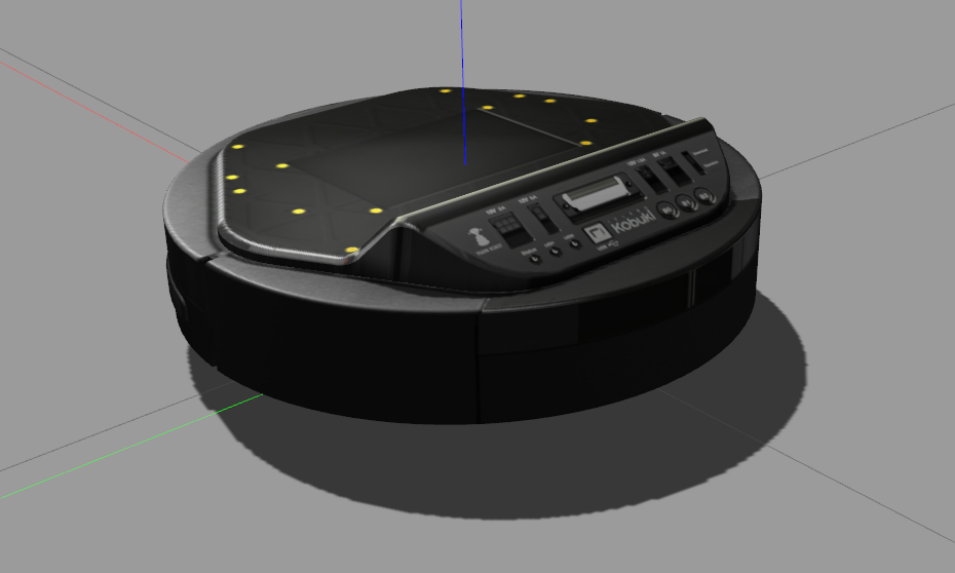
\includegraphics[width=10cm]{imagenes/cap4/sim_kobuki_base.png}
  \end{center}
  \caption[Modelo simulado Kobuki (ROS2)]{Modelo simulado Kobuki (ROS2)}
  \label{fig:sim_kobuki_base}
\end{figure}\



\subsection{Cuerpo del robot}
\label{subsec:cuerpo_simulado}

Aparte de la base Kobuki, la otra mitad que caracteriza al TurtleBot2 es la \textit{parte superior} o \textit{cuerpo} que permite colocar, sensores, actuadores o incluso portátiles (en los robots reales). En esta sección abordaremos su modelado y simulación con URDF y Xacro.\\

La pregunta es ¿por qué no usamos ficheros turtlebot\_description de la rama Noetic o Melodic si el lenguaje URDF es el mismo? En realidad, el paso de ROS a ROS2 conlleva cambios tanto en la manera de crear nodos, ficheros de lanzamiento y su funcionamiento interno como en el uso de URDF. El modelo TurtleBot2, al tener una gran cantidad de ficheros URDF que dependían unos de otros, y estos a su vez de otros paquetes con dependencias en ROS, no facilitaba la tarea de obtener un modelo creando únicamente ficheros de lanzamiento \texttt{launch.py} como hicimos con la base Kobuki.\\

La \textit{solución} fue crear la estructura restante del robot a mano, usando la sintáxis URDF y Xacro, diseñando un modelo lo más semejante posible al real. A continuación mostraremos las fases de desarrollo. Una vez terminado el modelo del TurtleBot2, tendremos por un lado un directorio con todos los paquetes de \textit{kobuki\_base} y otro directorio con la definición del nuevo soporte creado.\\

Usar Xacro permitió diseñar \textit{macros} que facilitaran la estructura y la legibilidad del modelo. Con Xacro está permitido incluir de manera sencilla, nuevos elementos en el modelo y establecer la jerarquía de transformadas entre \textit{links} de padres a hijos (siempre es importante indicar las relaciones jerárquicas para realizar futuras operaciones basadas en marcos de coordenadas).\\


Primero, en un fichero \texttt{structures.urdf.xacro} definimos dos macros para crear los \textit{links} que necesitamos y definimos las relaciones jerárquicas de padres a hijos. Las nuevas macros son \textit{cylinder\_structure} y \textit{cube\_structure}, para crear en el fichero \texttt{turtlebot2.urdf.xacro} elementos como los siguientes:\\
\begin{code}[H]
\begin{lstlisting}
<xacro:cylinder_structure name="base_tick5" x="0.15" y="0.0" z="0.14" length="0.15" radius="0.005" parent="base_link"/>
<xacro:cube_structure name="camera_support_base" x="0.13" y="0" z="0.0975" x_size="0.0175" y_size="0.15" z_size="0.005" parent="middle_base_link"/>
\end{lstlisting}
\caption{Creación de dos \textit{links} usando dos nuevas macros definidas (TurtleBot2 ROS Foxy)}
\label{fig:creacion_link_macro}
\end{code}

Después definimos en el fichero \texttt{colors.urdf.xacro} algunas macros para incluir colores en los \textit{links} del modelo de Gazebo:\\
\begin{code}[H]
\begin{lstlisting}
<xacro:macro name="create_color" params="name value">
	<material name="${name}">
		<color rgba="${value}"/>
	</material>
</xacro:macro>

<xacro:macro name="gazebo_color" params="link color">
	<gazebo reference="${link}">
		<material>Gazebo/${color}</material>
	</gazebo>
</xacro:macro>

<xacro:create_color name="Gray" value="0.5 0.5 0.5 1"/>
<xacro:gazebo_color link="base_tick1_link" color="Gray"/>
\end{lstlisting}
\caption{Creación y establecimiento de un color a un link}
\label{fig:creacion_color_link}
\end{code}\

Por útlimo, en el fichero \textit{turtlebot2.urdf.xacro} incluimos con la macro ``xacro:include" las definiciones URDF de los ficheros del paquete \textit{kobuki\_description}. Una vez llegados a este punto tendremos el robot TurtleBot2 simulado sin sensores. El siguiente paso es incorporar un láser de 360 grados y una cámara RGB-D.\\

Para la visualización del modelo URDF completo en Gazebo me basé en los mismos ficheros que hice con la base Kobuki: \texttt{empty\_world.launch.py} y \texttt{spawn\_model.launch.py} (Sección \ref{subsec:kobuki_base_simulado})\\

La única diferencia fue definir 3 argumentos por defecto para establecer la posición inicial del robot, y poder especificar el punto de partida cuando se quiera importar el modelo en cualquier otro mundo de Gazebo. Estos 3 argumentos se pasan al nodo \textit{spawn\_entity}. A continuación podemos ver la sección referente a la posición inicial del fichero \texttt{spawn\_model.launch.py}:\\

\begin{code}[H]
\begin{lstlisting}
	# Set (x, y, z) default position of turtlebot2
	x_pos = LaunchConfiguration('-x', default='0')
	y_pos = LaunchConfiguration('-y', default='0')
	z_pos = LaunchConfiguration('-z', default='0')
	
	spawn_entity_node = Node(
		package='gazebo_ros',
		executable='spawn_entity.py',
		name='entity_spawner',
		output='screen',
		arguments=["-topic", "/robot_description", "-entity", "turtlebot2", "-x", x_pos, "-y", y_pos, "-z", z_pos]
	)
\end{lstlisting}
\caption{Establecimiento de la posición por defecto del TurtleBot2 en el simulador}
\label{cod:posicion_defecto_turtlebot2_simulador}
\end{code}\

Para lanzar el robot en el simulador ejecutamos los siguientes comandos:\\
\begin{code}[H]
\begin{lstlisting}
ros2 launch turtlebot2 empty_world.launch.py &
ros2 launch turtlebot2 spawn_model.launch.py
\end{lstlisting}
\caption{Comandos para lanzar el robot TurtleBot2 en el simulador (ROS2 Foxy)}
\label{codd:comandos_turtlebot2_simulador}
\end{code}\

\begin{figure} [H]
  \begin{center}
    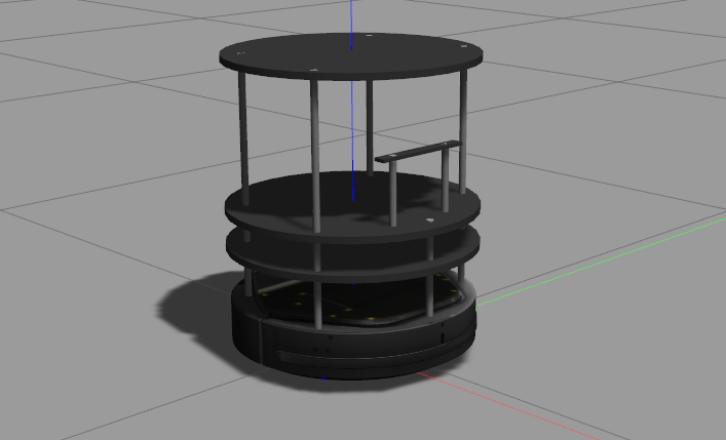
\includegraphics[width=10cm]{imagenes/cap4/cuerpo_turtlebot2.png}
  \end{center}
  \caption[Robot TurtleBot2 simulado sin sensores (ROS2 Foxy)]{Robot TurtleBot2 simulado sin sensores (ROS2 Foxy)}
  \label{fig:turtlebot2_sin_sensores_simulado}
\end{figure}\



\subsection{Sensores Láser y Cámara}
\label{subsec:sensores_camara}

Para usar un láser en Gazebo utilizamos un fichero .xacro que actuará como plantilla\footnote{\textbf{Láser Xacro}: \url{https://github.com/RoboticsLabURJC/2021-tfg-carlos-caminero/blob/main/turtlebot2/turtlebot2/urdf/sensors/lidar.urdf.xacro}} y permita posicionar el láser donde el programador quiera. En el fichero \texttt{lidar.urdf.xacro} indicamos algunas propiedades como el rango del láser, el ruido y el alcance.\\

Para colocar el sensor en el robot, tuvimos que incluir esta línea en el fichero \texttt{turtlebot2.urdf.xacro} donde indicamos su posición xyz y el \textit{link} padre:\\

\begin{code}[H]
\begin{lstlisting}
<xacro:set_lidar name="lidar" xyz="0 0 0.0275" parent_frame="upper_base_link"/>
\end{lstlisting}
\caption{Colocación del láser en el robot simulado}
\label{fig:colocacion_laser_simulado}
\end{code}\

Con la cámara RGB-D\footnote{\textbf{Cámara Xacro}: \url{https://github.com/RoboticsLabURJC/2021-tfg-carlos-caminero/blob/main/turtlebot2/turtlebot2/urdf/sensors/camera.urdf.xacro}} hicimos lo mismo. En su fichero Xacro \texttt{camera.urdf.xacro} definimos algunas propiedades como el alcance, el tamaño de los fotogramas o el \textit{campo de visión} (FOV).\\

Para colocar la cámara en el robot, tan solo teníamos que incluir esta línea en el fichero \texttt{turtlebot2.urdf.xacro} donde indicamos su posición xyz, su orientación y el \textit{link} padre:\\

\begin{code}[H]
\begin{lstlisting}
<xacro:set_camera name="camera" xyz="0.13 0 0.32" rpy="0 0 0" parent_frame="base_link"/>
\end{lstlisting}
\caption{Colocación de la cámara en el robot simulado}
\label{fig:colocacion_camara_simulado}
\end{code}\

Con esto, tendríamos todos los ficheros necesarios para usar el robot TurtleBot2 simulado completo. Con la incorporación de los sensores, su directorio quedó de la siguiente manera:

\begin{figure}[H]
	\begin{center}
	    \setlength{\fboxsep}{0.5cm}
	    \fbox{
        \begin{minipage}{10cm}
          \dirtree{%
          .1 turtlebot2.
          .2 kobuki\_base.
          .3 kobuki\_ros\_interfaces.
          .3 kobuki\_ros.
          .4 Ficheros de kobuki\_gazebo \ref{subsec:kobuki_base_simulado}.
          .4 \vdots.
          .2 turtlebot2.
          .3 launch.
          .4 empty\_world.launch.py.
          .4 spawn\_model.launch.py.
          .3 rviz.
          .3 urdf.
          .4 structures.urdf.xacro.
          .4 colors.urdf.xacro.
          .4 turtlebot2.urdf.xacro.
          .4 sensors.
          .5 camera.urdf.xacro.
          .5 lidar.urdf.xacro.
          .3 spawn.sh.
          .3 CMakeLists.txt.
          .3 package.xml.
          }
        \end{minipage}
        }
	    \caption{Estructura de directorios completa del Turtlebot2 (ROS2 Foxy)}
	    \label{fig:directorios_turtlebot2}
	\end{center}
\end{figure}\

En la figura \ref{fig:evolucion_turtlebot2_sim} podemos ver la evolución del proceso creativo del TurtleBot2 simulado hasta su resultado final:\\
\begin{figure} [H]
  \begin{center}
    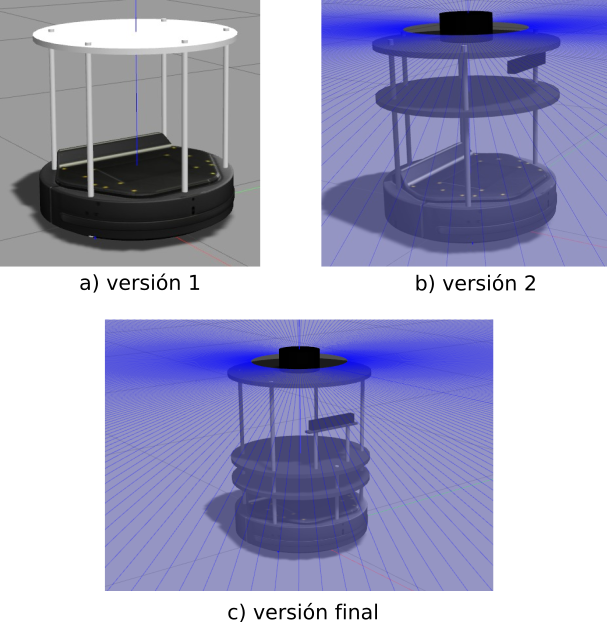
\includegraphics[width=12.5cm]{imagenes/cap4/creacion-turtlebot2-sim.png}
  \end{center}
  \caption[Evolución TurtleBot2 simulado]{Evolución TurtleBot2 simulado}
  \label{fig:evolucion_turtlebot2_sim}
\end{figure}\


\subsection{ROS topics}
\label{subsec:ros_topics}

Una vez que hemos descrito la parte mecánica del robot (modelo del TurtleBot2) es necesario incorporar \textit{drivers} que cojan datos de los sensores simulados y los ofrezcan en forma de \textit{topics} de ROS. Además, necesitaríamos incorporar \textit{drivers} que ofrezcan \textit{topics} con comandos de movimiento para enviarlo a los motores simulados. Para ello, usaremos los \textit{plugins} del simulador Gazebo 11.\\

Estos \textit{plugins} actúan como nodos ROS de manera homóloga a como actúan los drivers del robot real. Proporcionan los mismos \textit{topics} o parecidos compartiendo los mismos mensajes de transmisión. Los \textit{plugins} que ofrece Gazebo se incluyen en los ficheros URDF del robot:\\

\begin{itemize}
	\item En el fichero principal URDF de la base Kobuki: \texttt{kobuki\_gazebo.urdf.xacro} usamos el \textit{plugin} \texttt{libgazebo\_ros\_diff\_drive.so} para ofrecer un \textit{topic} llamado /cmd\_vel que permite comandar velocidades lineales y angulares a los motores.
	\item Para el láser del fichero \texttt{lidar.urdf.xacro} del TurtleBot2 usamos el \textit{plugin} \texttt{libgazebo\_ros\_ray\_sensor.so} que publica sobre un \textit{topic} llamado /scan las lecturas del láser.
	\item Para la cámara del TurtleBot2, usamos en el fichero \texttt{camera.urdf.xacro} el \textit{plugin} \texttt{libgazebo\_ros\_camera.so} que publica sobre un \textit{topic} llamado /depth\_camera/image\_raw los fotogramas que captura la cámara simulada.
\end{itemize}\

En la Tabla \ref{tab:ros_topics_turtlebot2_simulado} mostramos los \textit{topics} relevantes del TurtleBot2 simulado y cómo poder utilizarlos (mediante publicación o suscripción):

\begin{table}[H]
\begin{center}
\begin{tabular}{| c | c | c | c | }
\hline
\multicolumn{4}{ |c| }{\textbf{ROS topics TurtleBot 2 simulado}} \\ \hline
\textbf{Componente} & \textbf{Tipo} & \textbf{Topic} & \textbf{Mensaje} \\ \hline
Motores & Publicador & /cmd\_vel & geometry\_msgs.msg.Twist \\
Láser & Suscriptor & /scan & sensor\_msgs.msg.LaserScan \\
Cámara & Suscriptor & /depth\_camera/image\_raw & sensor\_msgs.msg.Image \\
Odometría & Suscriptor & /odom & nav\_msgs.msg.Odometry \\ \hline
\end{tabular}
\caption{ROS Topics TurtleBot2 simulado (ROS Foxy)}
\label{tab:ros_topics_turtlebot2_simulado}
\end{center}
\end{table}




\section{TurtleBot2 real}
\label{sec:robot_real_ros_foxy}

En esta sección nos centramos en los \textit{wrappers} para conectarnos a los \textit{drivers} del TurtleBot2 real usando ROS2 Foxy.\\

El desarrollo de \textit{Kobuki Core} en ROS2 se separó del repositorio original originando un cambio de dirección URL\footnote{\textbf{Drivers Kobuki (ROS2)}: \url{https://github.com/kobuki-base/kobuki_core}}. Para controlar la base Kobuki usamos el repositorio \textit{Kobuki\_ROS}\footnote{\textbf{Wrapper Kobuki (ROS2)}: \url{https://github.com/kobuki-base/kobuki_ros}} (el mismo que usamos en la sección \ref{subsec:kobuki_base_simulado} para usar el paquete \textit{kobuki\_description} que actúa de \textit{wrapper} conteniendo los paquetes \textit{kobuki\_node} y \textit{kobuki\_keyop}:\\

\begin{itemize}
	\item \textbf{kobuki node}: Es el paquete que contiene un fichero de configuración denominado \texttt{kobuki\_node\_params.yaml} con el que podemos conectarnos al robot real usando el puerto /dev/ttyUSB0, así como la definición de algunos marcos de coordenadas (base, odom). También contiene los ficheros de los nodos necesarios para controlar la base Kobuki y su odometría. Oculta al programador la complejidad de comunicarse directamente con el hardware (motores, leds...) del robot usando nodos ROS (mediante publicadores y suscriptores). El nodo que lanza \textit{kobuki\_ros\_node} se suscribe al \textit{topic} /commands/velocity para recibir mensajes de tipo \textit{geometry\_msgs.msg.Twist} y poder mover mediante velocidad lineal y angular la base del robot. Este directorio no tiene relación con \textit{kobuki\_description}.
	\item \textbf{kobuki\_keyop}: Es un paquete que permite mover la base del robot con el teclado del ordenador. Se crea un nodo que publica por cada pulsación del teclado, un mensaje geometry\_msgs.msg.Twist en el \textit{topic} \textit{/cmd\_vel} (tendremos que cambiar a \textit{/commands/velocity} si queremos controlar el robot real. Este paquete puede ayudar en un principio a comprobar que tenemos conexión con el hardware real.
\end{itemize}\

Para usar el láser RPLIDAR A1 en la distribución Foxy se ha usado el repositorio \textit{rplidar\_ros}\footnote{\textbf{rplidar\_ros (ROS2)}: \url{https://github.com/allenh1/rplidar_ros}} del usuario de Github \textit{allenh1} en su rama para ROS2, cuyo fichero de lanzamiento \texttt{rplidar.launch.py} permite recoger lecturas con el sensor.\\

La cámara IntelRealsense R200 no tenía soporte para ROS2 y por lo tanto, no podíamos aprovecharnos de sus características (profundidad). De modo que hemos usado el paquete de ROS2 \textit{v4l2-camera} que sirve para publicar sobre un \textit{topic} llamado (/image\_raw) las imágenes que captura la cámara a una frecuencia de 60 Hz.\\

Con los drivers de la base Kobuki, el láser y la cámara tenemos todo lo necesario para usar la distribución Foxy en el robot real. En la Tabla \ref{tab:ros_topics_turtlebot2_real} mostramos los ROS topics que usa el robot. Como podréis ver, algunos topics han cambiado, de modo que lo hemos tenido en cuenta para la creación de los ejercicios.\\

\begin{table}[H]
\begin{center}
\begin{tabular}{| c | c | c | c | }
\hline
\multicolumn{4}{ |c| }{\textbf{ROS topics TurtleBot 2 real}} \\ \hline
\textbf{Componente} & \textbf{Tipo} & \textbf{Topic} & \textbf{Mensaje} \\ \hline
Motores & Publicador & /commands/velocity & geometry\_msgs.msg.Twist \\
Láser & Suscriptor & /scan & sensor\_msgs.msg.LaserScan \\
Cámara & Suscriptor & /image\_raw & sensor\_msgs.msg.Image \\
Odometría & Suscriptor & /odom & nav\_msgs.msg.Odometry \\ \hline
\end{tabular}
\caption{ROS Topics TurtleBot2 real (ROS Foxy)}
\label{tab:ros_topics_turtlebot2_real}
\end{center}
\end{table}

Cuando publicamos en \textit{/commands/velocity} el nodo de la base Kobuki (fichero \texttt{kobuki\_ros.cpp} del paquete \textit{kobuki\_node}) se suscribe al topic y comanda directamente las velocidades al hardware: \textit{kobuki\_.setBaseControl(msg-$>$linear.x, msg-$>$angular.z)}





\section{Integración en el RADI 4}
\label{sec:robot_radi4}

Para integrar el TurtleBot2 simulado y real en Robotics Academy se ha empezado creando una rama externa de desarrollo\footnote{\textbf{RADI-prueba}: \url{https://github.com/Carlosalpha1/RoboticsAcademy/tree/test-radi}} donde se ha ido realizando varias pruebas con el contenedor Docker. Para su integración hemos usado los ficheros \textit{Dockerfile} del RADI 4 donde hemos especificado los comandos necesarios para su instalación y soporte\\

En el repositorio de terceros CustomRobots, subimos el soporte del robot\footnote{\textbf{Custom Robots TB2}: \url{https://github.com/JdeRobot/CustomRobots/tree/foxy-devel/turtlebot2}} tanto real como simulado, con algunas dependencias necesarias: \textit{Kobuki\_ros} modificado, \textit{kobuki\_ros\_interfaces} y el diseño del cuerpo del robot. Por tanto, en el Dockerfile clonamos la rama \textit{foxy-devel} de dicho repositorio. Además, instalamos algunos paquetes extras que son necesarios para la compilación del espacio de trabajo:

\begin{code}[H]
\begin{lstlisting}
# Follow Person: Turtlebot2 dependencies
RUN apt-get update && apt-get -y --quiet --no-install-recommends install \
    ros-$ROS_DISTRO-ecl-build \
    ros-$ROS_DISTRO-diagnostic-updater \
    ros-$ROS_DISTRO-kobuki-core \
    ros-$ROS_DISTRO-ecl-errors \
    ros-$ROS_DISTRO-ecl-exceptions \
    ros-$ROS_DISTRO-ecl-geometry \
    ros-$ROS_DISTRO-ecl-linear-algebra \
    ros-$ROS_DISTRO-ecl-sigslots \
    ros-$ROS_DISTRO-joint-state-publisher \
    ros-$ROS_DISTRO-v4l2-camera \
  && apt-get -y autoremove \
  && apt-get clean autoclean \
  && rm -rf /var/lib/apt/lists/{apt,dpkg,cache,log} /tmp/* /var/tmp/*
\end{lstlisting}
\caption{Instalación de dependencias para el TurtleBot2 (Dockerfile.base)}
\label{fig:instalacion_dependencias_turtlebot2_dockerfile_base}
\end{code}\

\begin{code}[H]
\begin{lstlisting}
# Custom Robot Repository
RUN mkdir -p /opt/jderobot && cd /opt/jderobot && \
  git clone -b $ROS_DISTRO-devel https://github.com/JdeRobot/CustomRobots.git

# Adding RPLIDAR ROS
RUN cd /opt/jderobot/CustomRobots && \
  git clone https://github.com/allenh1/rplidar_ros.git -b ros2 && \
  cd rplidar_ros/launch && \
  sed -i "$(grep -n serial_port rplidar.launch.py | cut -d: -f1) s/\/dev\/ttyUSB0/\/dev\/ttyUSB1/g" rplidar.launch.py
\end{lstlisting}
\caption{Instalación de dependencias para el TurtleBot2 (Dockerfile)}
\label{fig:instalacion_dependencias_turtlebot2_dockerfile}
\end{code}

Para el láser hemos cambiado en el fichero \textit{rplidar.launch.py} el puerto /dev/ttyUSB0 por /dev/ttyUSB1 usando el comando de Linux \textit{sed} ya que la base Kobuki usa /dev/ttyUSB0 por defecto.\\

Una vez instaladas las dependencias y construida la imagen Docker, se han de tener en cuenta los dispositivos conectados en el portátil del usuario para el lanzamiento del contenedor. Para indicar al contenedor qué dispositivos del sistema operativo queremos integrar dentro del sistema virtualizado usaremos el parámetro \textit{--device}. Cuando usemos el robot real, tendremos que seguir las siguientes reglas en el siguiente orden (preferiblemente):\\

\begin{itemize}
	\item \textbf{Base Kobuki}. Al encender la base Kobuki y conectarla al portátil, su conexión abrirá el dispositivo /dev/ttyUSB0.
	\item \textbf{RPLIDAR A1}. Al conectar su cable USB \textit{después} de conectar la base Kobuki se habilitará el dispositivo /dev/ttyUSB1.
	\item \textbf{Cámara Intel Realsense R200}. Su conexión abré 6 dispositivos /dev/video[0-5]. Nosotros nos quedamos con /dev/video4 cuya salida se muestra en el espacio de color RGB (comprobado con este comando \footnote{\textbf{cvlc v4l2:///dev/video4}}). Como se ha integrado en Robotics Academy para las cámara que abran el dispositivo /dev/video0 tendremos que usar un remapeo: /dev/video4:/dev/video0.
\end{itemize}\

El comando para lanzar el RADI 4 usando la cámara R200 será el siguiente (para otras cámaras el remapeo puede ser distinto):\\

\begin{code}[H]
\begin{lstlisting}
$>  docker run -it --rm --device /dev/ttyUSB0 --device /dev/ttyUSB1 --device /dev/video4:/dev/video0 -p 8000:8000 -p 2303:2303 -p 1905:1905 -p 8765:8765 -p 6080:6080 -p 1108:1108 jderobot/robotics-academy:4.3.0 ./start.sh
\end{lstlisting}
\caption{Lanzamiento del RADI 4 con el robot real}
\label{cod:lanzamiento_radi_robot_real}
\end{code}\

Si usamos el robot simulado, no necesitaremos los puertos USB físicos citados anteriormente. De manera opcional podremos usar el parámetro \textit{--device /dev/dri} para habilitar la aceleración gráfica y mejorar así el rendimiento en FPS de la simulación.\\

En el siguiente capítulo, nos centraremos de la construcción de los nuevos ejercicios que usan respectivamente el soporte del robot TurtleBot2 simulado y del TurtleBot2 físico que hemos descrito en este capítulo.


%\textbf{Consideraciones a tener en cuenta}: Tanto el modelo Kobuki como el Turtlebot 2 simulado usan un plugin para controlar los motores denominado \textit{differential\_drive\_controller.so}. Este plugin se suscribe a un topic para controlar la velocidad de las ruedas del robot llamado /cmd\_vel (estándar en ROS), por lo que no coincide con el topic del robot real /commands/velocity.


